\section{Fast Coresets in Practice}

We now provide an experimental analysis to verify that (1) Fast-Coresets obtain solutions of equal quality to sensitivity sampling while running significantly
faster, and (2) of the linear-time algorithms, only Fast-Coresets are guaranteed to satisfy the coreset property. We proceed by first
introducing our experimental setup, including the metrics, datasets, and algorithms being analyzed. We then follow this by a discussion of results regarding
both of the above claims.

\subsection{Experimental Setup}
\subsubsection{Metrics}

We analyze the coreset construction methods along two metrics -- coreset quality and construction time.  Although measuring runtime is standard, predicting coreset
quality is a more difficult task. Specifically, it is unclear how to confirm that a subset of points satisfies the coreset property over all solutions. To this
end, we use the following distortion measure
\[ \max \left( \dfrac{\cost(P, \calC_{\Omega})}{\cost(\Omega, \calC_{\Omega})}, \dfrac{\cost(\Omega, \calC_{\Omega})}{\cost(P, \calC_{\Omega})} \right),\]
where $\calC_{\Omega}$ is a candidate solution that was computed over the coreset~\cite{chrisESA}. This will be within
$1+\varepsilon$ if the coreset guarantee is satisfied but may be unbounded otherwise. 

We refer to this metric as the \emph{coreset distortion}. Naturally, values that are consistently close to $1$ suggest that solutions on the coreset are likely
viable on the full dataset.


\subsubsection{Algorithms}
\label{ssec:algorithms}

\chris{Not to say we should plagiarize, but can we write this similar to the ESA paper? In general I found the ESA paper had a lot more detail. Also, a number of the comments are wrong or misleading. BICO does not use BIRCH.}

We compare our method (Algorithm~\ref{alg:main}) against 5 different benchmark coreset constructions:
\begin{itemize}
        \item \emph{Standard uniform sampling}. Uniform coresets are obtained by choosing a subset of $m \ll n$ points uniformly from $P$.
        \item \emph{Lightweight coreset}. Lightweight coresets find the mean $\mu$ of the dataset and obtain per-point sensitivity estimates by $\hat{s}(p) = 1/|P| + \cost(p, \mu) / \cost(P, \mu)$.
            The first term encourages uniform sampling while the second encourages sampling proportionate to the importance. In the setting where the mean is
            a constant-factor approximation of the optimum, this is akin to sensitivity sampling.
        \item \emph{Birch using Coresets (BICO)}: BICO utilizes the fast hierarchical clustering algorithm BIRCH~\cite{birch} to find a coreset using the
            triangle inequality with resepect to the centers. BICO has an exponential dependency on $d$, making it a poor candidate for high-dimensional datasets.
        \item \emph{Standard sensitivity sampling}. We follow the standard approach for sensitivity sampling outlined in Section~\ref{ssec:sens_sampling}.
        \item \emph{Welterweight coreset}: This is a generalized interpolation between lightweight coresets and the `heavy-duty' sensitivity sampling coresets. For any $j
            \in \{1,..., k\}$, we compute a coreset using sensitivity sampling with respect to a candidate $j$-means++ solution. For values $j \leq O(\log k)$,
            welterweight coresets share the runtime complexity of Fast-Coresets.
\end{itemize}
All but BICO have been implemented by us in a single codebase. We use the BICO code from \cite{bico}.

We take a moment here to motivate the welterweight coreset algorithm.  Consider that lightweight coresets are simply solving $1$-means to obtain sensitivity
values whereas sensitivity sampling is solving the $k$-means problem. Since the lightweight coreset has the advantage of being fast while sensitivity sampling
is more precise, one could hope to interpolate in order to get the best of the two worlds: computing an approximate $j$-means solution may allow to obtain
a more precise sampling distribution than that of lightweight-coresets, while being faster than sensitivity sampling. We analyze the different choices of $j$ in
Table~\ref{tbl:class-imbalance} and default to $j = \log k$ in the other experiments.

\subsubsection{Datasets}

We employ several real and artificial datasets to evaluate the quality of a coreset. 

For our real-world data, we utilize the Adult~\cite{Dua:2019}, MNIST~\cite{mnist}, Song~\cite{song}, Census~\cite{census}, and Cover Type~\cite{covtype}
datasets, whose characteristics are summarized in Table~\ref{tbl:datasets} below.

\begin{table}[htbp]
    \centering
    \begin{tabular}{lrr}
        Dataset & Points & Dim \\
        \hline
        \emph{Adult} & 48\,842 & 14 \\
        \emph{MNIST} & 60\,000 & 784 \\
        \emph{Song} & 515\,345 & 90 \\
        \emph{Cover Type} & 581\,012 & 54 \\
        \emph{Census} & 2\,458\,285 & 68
    \end{tabular}
    \caption{Description of real world datasets}
        \label{tbl:datasets}
\end{table}

To complement those, we use several artificial datasets, each controlling for one relevant dataset attribute. Unless stated otherwise, $n = 50\,000$
and $d=50$.
\begin{itemize}
    \item \emph{c-outlier}. Place $n-c$ points in a single location and $c$ points placed at a large distance away, for some constant $c$. We default to $c=5$.

    \item \emph{Gaussian mixture}.  Multivariate Gaussians with varying cardinalities arranged randomly in high-dimensional space.  Each cluster has a center
        sampled from a multivariate normal with mean $0$ and variance $1\,000$ and each cluster is then i.i.d. samples multivariate normal distribution around
        this mean. Cluster sizes are defined as the random variable $|C_i| = \frac{n}{\kappa} \exp \left( \gamma(\rho_i - \frac{1}{2}) \right)$, where $\kappa$
        is the number of Gaussian clusters, $\rho_i$ is a uniform random variable, and $\gamma$ is a chosen hyperparameter\footnote{We show the effect of
        $\gamma$ on the cluster distribution in Figure~\ref{fig:effect-of-gamma}}. We obtain each cluster iteratively: once we have sampled one cluster of size
        $|C_0|$, we repeat the process for the next cluster with $|C_1| = \frac{n - |C_0|}{\kappa-1}\exp \left( \gamma(\rho_1 - \frac{1}{2}) \right)$.  Thus,
        each cluster has size $\frac{n}{k}$ when $\gamma = 0$ and the cluster sizes diverge as $\gamma$ grows. We default to $\gamma = 5$.

    \item \emph{Geometric}. Place $c k$ points at $(1, 0, 0, \cdots)$, $\frac{ck}{r}$ points at $(0, 1, 0, \cdots)$, $\frac{ck}{r^2}$ points
        at $(0, 0, 1, \cdots)$, and so on for $\log_r (ck)$ rounds. Thus, the data creates a high-dimensional simplex with uneven weights across the vertices. We
        default to $c = 100$ and $r=2$. 

    \item \emph{Benchmark}. A specific distribution of points introduced in \cite{chrisESA} as a good testbed for coreset algorithms.  It has the property that
        all reasonable $k$-means solutions are of equal quality but are maximally far apart in the solution space. Thus, the dataset is fully determined by the
        number of centers $k$. We follow the advice in the benchmark's original presentation and produce three benchmark datasets of varying size before
        applying random offsets to each. We choose the sizes by $k_1 = \frac{k}{c_1}$, $k_2 = \frac{k - k_1}{c_2}$, and $k_3 = k - k_1 - k_2$ for $c_1, c_2 \in
        \mathbb{Z}$.

\end{itemize}

In all real and artificial datasets, we add random uniform noise $\eta$ with $0 \leq \eta_i \leq 0.001$ in each dimension in order to make all points unique.
Unless specifically varying these parameters, we default all algorithms in~\ref{ssec:algorithms} to $k=100$ for the Adult, MNIST, and artificial datasets and
$k=500$ for the Song, Cover Type, and Census datasets. Our default coreset size is then $m = 40k$. We refer to the coreset size scalar as the \emph{$m$-scalar}.
We only run the dimension-reduction step on the MNIST dataset, as the remaining datasets already have sufficiently low dimensionality.

\andrew{Add implementation details, machine specifics, etc.}

\subsection{Comparing Fast-Coresets to the State of the Art}
\label{ssec:alg_qualities}


\paragraph*{Comparison with standard sensitivity sampling.}

\begin{figure*}
\label{fig:coreset_size_on_sens_quality}
\centering
\begin{tabular}{lc}
    \rotatebox[origin=l]{90}{\bf \;\quad\quad\quad\quad\quad\quad\quad$k$-Median} &
    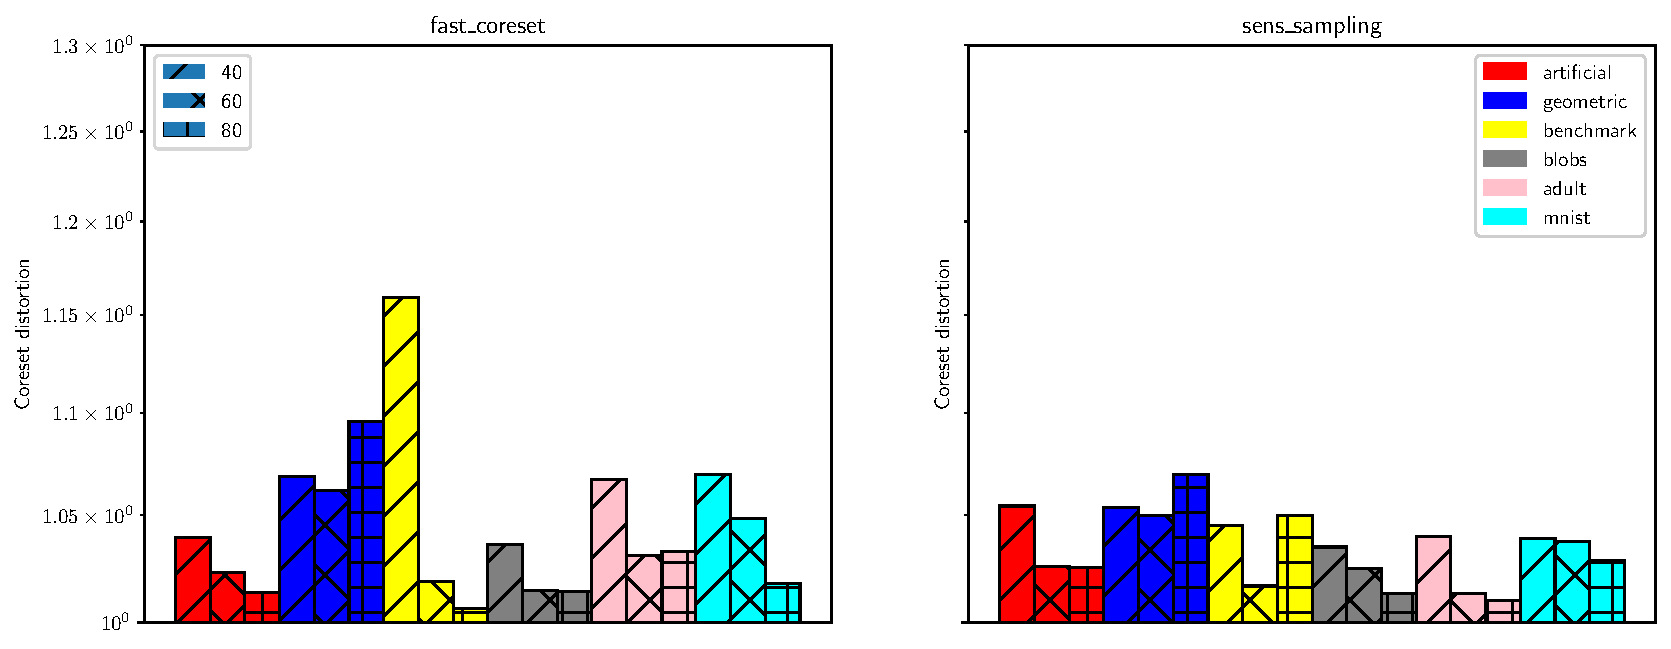
\includegraphics[width=.95\linewidth]{images/1/coreset_distortion-m_scalar_for_sens_sampling.pdf} \\

    \rotatebox[origin=l]{90}{\bf \;\;\quad\quad\quad\quad\quad\quad\quad$k$-Means} &
    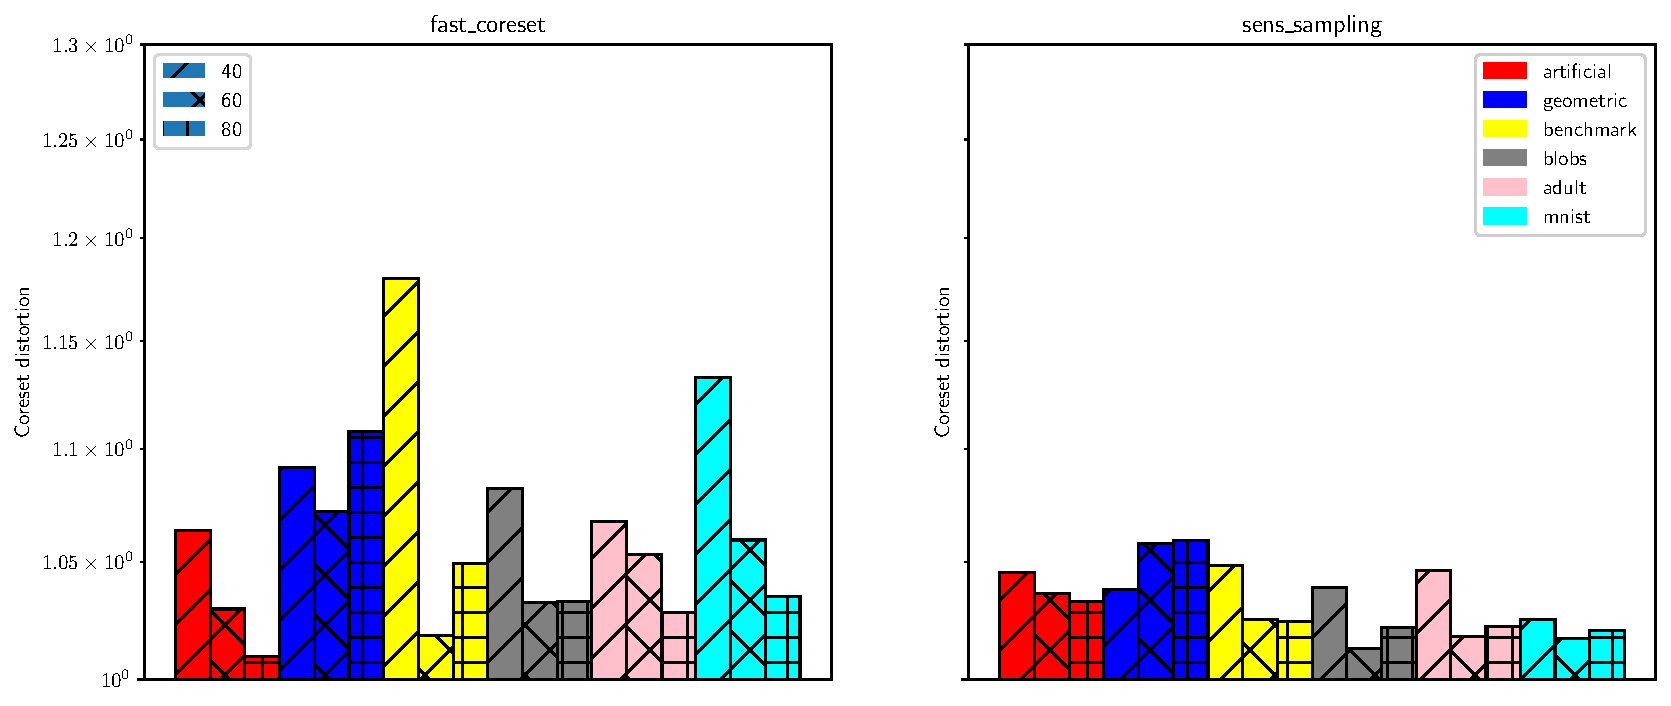
\includegraphics[width=.95\linewidth]{images/2/coreset_distortion-m_scalar_for_sens_sampling.pdf}
\end{tabular}
\caption{The effect of the coreset size on the distortion metric for sensitivity sampling approaches.
We point out that all distortion values are well below $\varepsilon = 0.2$.
Thus, for sufficient coreset sizes, there does not seem to be a meaningful difference between using Fast-Kmeans++ vs. regular Kmeans++.}
\end{figure*}


We first compare the Fast-Coreset algorithm with standard sensitivity sampling in terms of both quality and runtime.  To this end, the top of
Figure~\ref{fig:coreset_size_on_sens_quality} shows that, across datasets, the Fast-Coreset method produces coresets of consistent quality. Specifically, we
vary the $m$-scalar parameter and see that all distortion values are below $1.2$. Furthermore, choosing a sufficient coreset size ($m$-scalar$=80$) gives
distortion below $1.03$ for both Fast-Coresets and traditional sensitivity sampling. Despite this, we see in the bottom of Figure~\ref{fig:k_on_runtime} that
varying $k$ from $50$ to $400$ causes a linear slowdown in sensitivity sampling but only a logarithmic one for the Fast-Coreset method.

\andrew{Should this paragraph be here or with the artificial dataset discussion?}
We take a moment to discuss the Fast-Coreset algorithm's results on the particularly challenging benchmark and geometric datasets. First, consider that these
datasets are purposefully difficult, as the sensitivities are awkward to approximate and the clusters have unequal numbers of points.
Furthermore, the nature of the constructions leads to highly varying densities across the dataset, imposing an extra challenge on the HST metric-embeddings.
Despite these obstacles, we see that the Fast-Coreset method manages to find a low-distortion compression for reasonable coreset sizes ($m$-scalar$=80$).

This analysis confirms the theory predicted by \cref{thm:main}: Fast-Coresets run with little overhead while retaining the accuracy of sensitivity sampling.
Given this context, we did not add traditional sensitivity sampling to further experiments, as it is infeasible to run on large datasets.


\paragraph*{Comparison with other coreset methods.}

We now refer the reader to Figure~\ref{fig:coreset_size_on_quality}, where we show the effect of coreset size on the distortion across datasets and methods by
sweeping over $m$-scalar values in $[20, 40, 60, 80]$. 
First, we note that BICO performs poorly on all datasets -- even worse than uniform sampling.
Second, as expected, uniform sampling fails catastrophically on the artifical datasets due to the low likelihood of hitting all of the points.
Lastly, we see that, as expected, coresets of larger size obtain lower distortion across datasets.

We take a moment to comment on the more involved coreset constructions, lightweight and Cut-$k$-means. The Cut-$k$-means coreset surprisingly does not perform better than
lightweight coresets. Our tentative explanation for this lies in the reason why lightweight performs well on some dataset: those are rather uniform instances, well
spread around their means, with clusters of equivalent sizes. \david{not sure it is true} Sampling according to distance to the mean makes therefore sense,
while sampling according to a $j$-means solution (for small $j$) actually introduces bias against points close to the centers of that solution.  Furthermore,
lightweight coreset performs bad when there are $k$ unbalanced clusters, as illustrated in the gaussian-mixture dataset, as in
Figure~\ref{fig:lightweight_breaks}.  Our artificial dataset emphasize this effect, which does not appear in the real-world dataset (probably due to our choice
of large $k$) but is very plausible.  \david{add precise comments, depending on the actual precision of the coreset, especially for lightweight. }
\andrew{I'm not sure what to do with this paragraph. On the one hand, I agree that we should discuss it. On the other hand, I am wary of giving handwavy
explanations without evidence to back them up. Chris, what do you think?}
\david{Agreed on the handwaving -- although interpreting experiments is always somewhat handwavy I guess. Chris?}

\begin{figure}
\centering
\begin{tabular}{lc}
    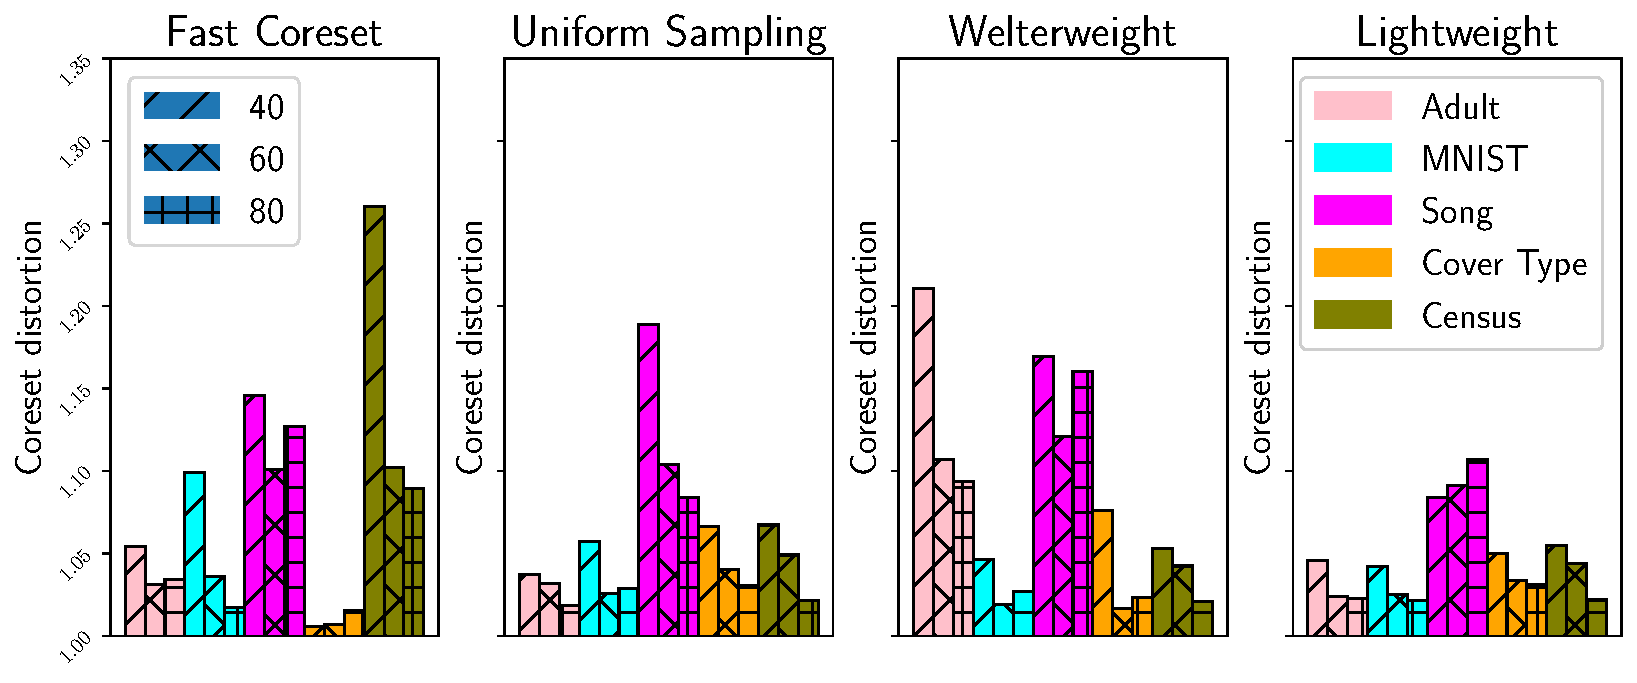
\includegraphics[width=\linewidth]{images/distortion_real_data} \\
    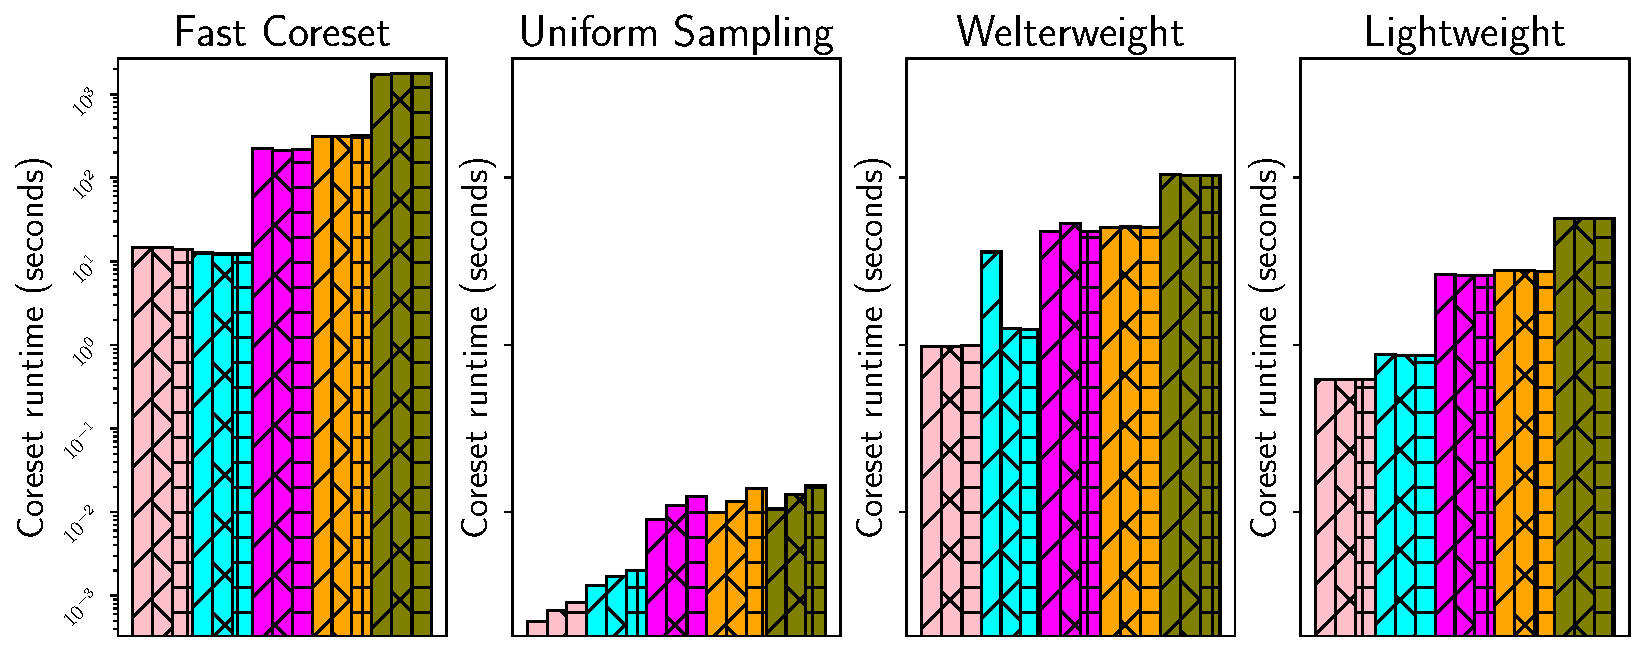
\includegraphics[width=\linewidth]{images/runtime_real_data}
\end{tabular}

\caption{\emph{Top}: The effect of the $m$-scalar on coreset distortion for real-world datasets. This is a visualization of the data in
Table~\ref{tbl:distortion}.  \emph{Bottom}: The effect of the $m$-scalar on the algorithm runtime for real-world datasets. All values are the mean over 5 runs.
The three bars represent samples of size $m=40k, 60k, 80k$.}

\label{fig:coreset_size_on_quality}
\end{figure}


\paragraph*{Additional evaluation on imbalanced clusters.}

\begin{table*}[htbp]
    \centering
    \small
    \begin{tabular}{|c|cccc|cccc|cccc|cccc|}
        \hline
        & \multicolumn{16}{c|}{Method} \\
        \cline{2-17}
        & \multicolumn{4}{c|}{Uniform Sampling} & \multicolumn{4}{c|}{Lightweight} & \multicolumn{4}{c|}{Welterweight} & \multicolumn{4}{c|}{Fast Coreset} \\
        %\cline{2-17}
        % & \multicolumn{4}{c|}{Coreset Size} & \multicolumn{4}{c|}{Coreset Size} & \multicolumn{4}{c|}{Coreset Size} & \multicolumn{4}{c|}{Coreset Size} \\
        & $20k$ & $40k$ & $60k$ & $80k$ & $20k$ & $40k$ & $60k$ & $80k$ & $20k$ & $40k$ & $60k$ & $80k$ & $20k$ & $40k$ & $60k$ & $80k$ \\
        \cline{2-17}
        $c$-outlier & 710 & 126 & 488 & 89.4 & 1.09 & 1.04 & 34.3 & 1.02 & 1.09 & 1.04 & 21.8 & 34.3 & 1.12 & 1.05 & 1.03 & 1.02 \\
        Gaussian Mix. & 1.09 & 1.03 & 1.03 & 1.01 & 204 & 86.1 & 84.3 & 1.01 & 617 & 16.8 & 8.18 & 13.3 & 1.22 & 1.03 & 1.02 & 1.01 \\
        Geometric & 89.4 & 107 & 31.4 & 61.8 & 163 & 13.3 & 50.4 & 1.02 & 1.28 & 1.08 & 1.07 & 19.2 & 1.17 & 1.09 & 1.09 & 1.09 \\
        Benchmark & 1.09 & 1.04 & 1.04 & 1.03 & 1.14 & 1.05 & 1.05 & 1.03 & 1.12 & 1.05 & 1.06 & 1.04 & 1.54 & 1.35 & 1.14 & 1.02 \\
        \hline
    \end{tabular}
\end{table*}

\begin{table}[htbp]
    \centering
    \begin{tabular}{lcccc}
        Algorithm & $\gamma = 0$ & $\gamma = 1$ & $\gamma = 3$ & $\gamma = 5$\\
        \hline
        LW Coreset & 1.03 & 1.03 & 1.36 & 2.17\\
        $j=2$ & 1.04 & 1.04 & 1.04 & 1.92\\
        $j=\log k$ & 1.04 & 1.04 & 1.04 & 1.95\\
        $j=\sqrt{k}$ & 1.05 & 1.06 & 1.04 & 1.18\\
        Fast Coreset & 1.03 & 1.03 & 1.04 & 1.12
    \end{tabular}
    \caption{The effect of $\gamma$ in the Gaussian mixture dataset on the coreset distortion. We report the means over 5 random dataset generations.
    Each generation had 50\,000 points in 50 dimensions, with 50 Gaussian clusters and coresets of size 4\,000. We set $k=100$.}
        \label{tbl:class-imbalance}
\end{table}
\begin{figure}[htbp]
    \centering
    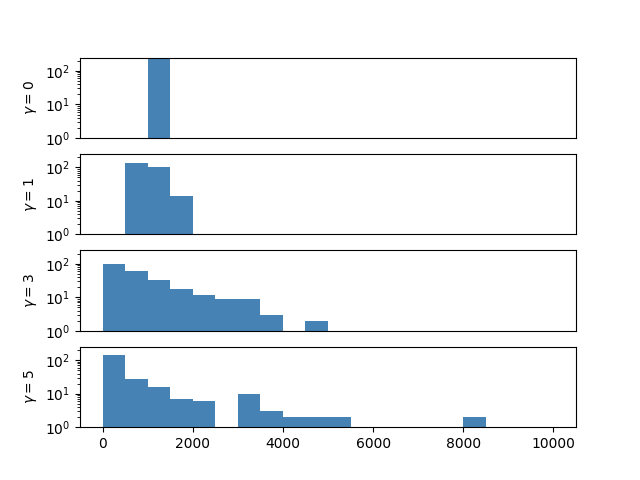
\includegraphics[width=\linewidth]{images/effect_of_gamma.png}
    \caption{Histograms of cluster sizes for different values of $\gamma$ in the Gaussian mixture dataset.}
        \label{fig:effect-of-gamma}
\end{figure}

\david{Say what is the coreset size. Do you know why is Fast Coreset so bad as well? Would it be possible to increase it to have a good fast coreset?}
\andrew{Are you asking why the fast coreset performs poorly in table~\ref{tbl:class-imbalance}? I think it does okay\ldots -- I can mention that this is for
$m=20k$, which is a small coreset. I used a small one to emphasize the difference but can use a bigger one so that our scores aren't as bad.}
\david{Ok, I didn't know the size was so small -- Yes, maybe a bigger one would be great (to be able to claim that fast coreset is consistently below 1.05 or something}

As discussed, the sensitivities for lightweight coresets are obtained by a linear combination of a uniform distribution and each point's relative
distance to the mean. Since the Gaussian mixture dataset has clusters of varying sizes, a small cluster that is close to the mean is unlikely
to ever be sampled. We argue that, although this is a toy dataset, one can easily imagine real-world datasets that have this property. 
As a simple solution, we see that the Cut-$k$-means coreset obtains satisfactory solutions on the Gaussian mixture dataset for 
\david{I don't know what you meant unfortunately}
\andrew{I have not gotten to changing this paragraph, but it will basically say that the table of class imbalance shows that, as class imbalance grows, it is
better to have $j>1$. I intend to add other values of $\gamma$ to that table.}

A similar argument can be made for the more-challenging geometric dataset, where the cluster size decreases exponentially and all clusters are equidistant.
We show furthermore that, for small values of $j$, sensitivities obtained according to
solutions for $j$-means are insufficient to create a coreset for the geometric-progression dataset.

To further measure the effect that the class imbalance has on the quality of each coreset, we define a class imbalance parameter $\gamma$ and obtain each
cluster's size by 
\begin{figure*}
\label{fig:lightweight_breaks}
\centering
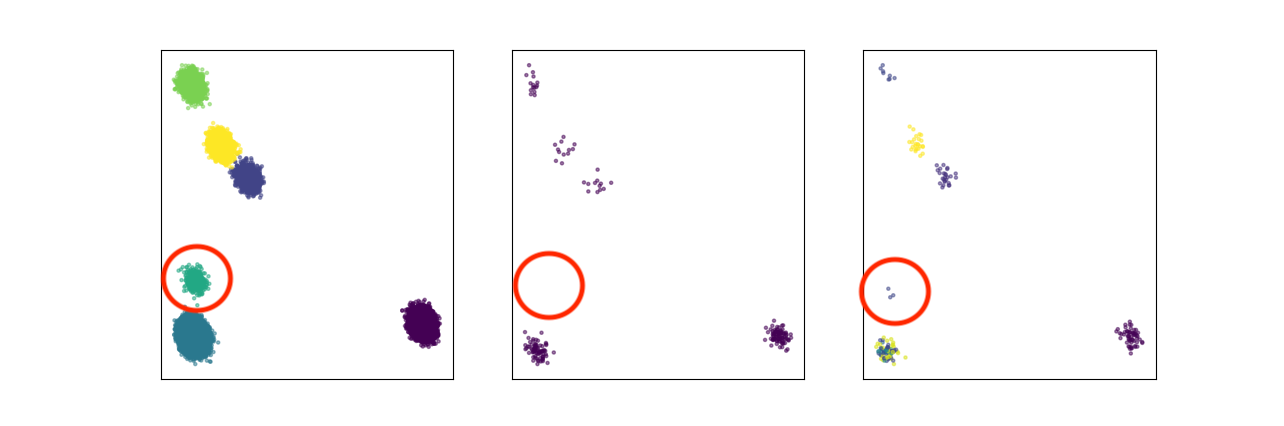
\includegraphics[width=.95\linewidth]{images/lightweight_breaks.png}
\caption{
The results of lightweight and fast-coreset constructions on a dataset of $n=100K$ points with clusters of varying size. Coresets have 200 points.
\emph{Left}: Original multivariate-Gaussian dataset. \emph{Middle}: Lightweight coresets fail to capture the cluster of $\sim$400 points.
\emph{Right}: The Fast-coreset construction runs in linear time but identifies all of the clusters.
}
\end{figure*}


We see the effect of $\gamma$ on the coreset distortion in Table~\ref{tbl:class-imbalance}, where even
small values of $\gamma$ can break the lightweight coreset construction.   Looking at the sensitivities computed via $j$-means++, we see that using $(j>1)$ is better at maintaining the coreset
property for higher values of $\gamma$ but is still not guaranteed to obtain satisfactory compression. Despite this, sensitivity sampling consistently obtains
coresets with low distortion.

\david{the sentence "cluster sizes diverge exponentially as $\gamma$ grows linearly"
is not super clear to me, because of the randomness. Also, since you are only showing two values of $\gamma$, it is hard to say that "it grows linearly": would
it be possible to add the ratio max size / min size for $\gamma = 5$ ? This should be something close to $\exp(10)$ which is crazy huge compared to $50000$, so
maybe not the right thing to plot...}
\andrew{If I'm understanding correctly, you're saying that we should add a value for the largest cluster size divided by the smallest cluster size? I'm happy to
do that. I think we could also just say what it is in expectation.}

